%%This is a very basic article template.
%%There is just one section and two subsections.
\documentclass{article}

\usepackage{a4wide}
\usepackage{amsmath}
\usepackage{float}
\usepackage{listings}
\usepackage{graphicx}
\usepackage{epstopdf}

\lstset{ %
breaklines=true,
language=R
}

\begin{document}

\title{Probability and Statistics for Data Analysis\\Assignment 2}
\author{Charalampos Kaidos}

\maketitle

\section{}
In the spreadsheet named Data 1 of the file Assignment 3 data.xlsx (available on
e-class assignments site) you will find the recorded variables $Y, X_1, X_2,
X_3$ (continuous) and $W$ (categorical with three levels) on 150 cases. Using
these data answer the following questions:

\subsection{}
Run the parametric one-way ANOVA of each of the continuous variables ($Y, X_1,
X_2, X_3$) on the categorical variable ($W$). Specifically,

\subsubsection{}
Provide a graphical representation of each of the continuous versus the
categorical variable

\begin{figure}[H]
\centering
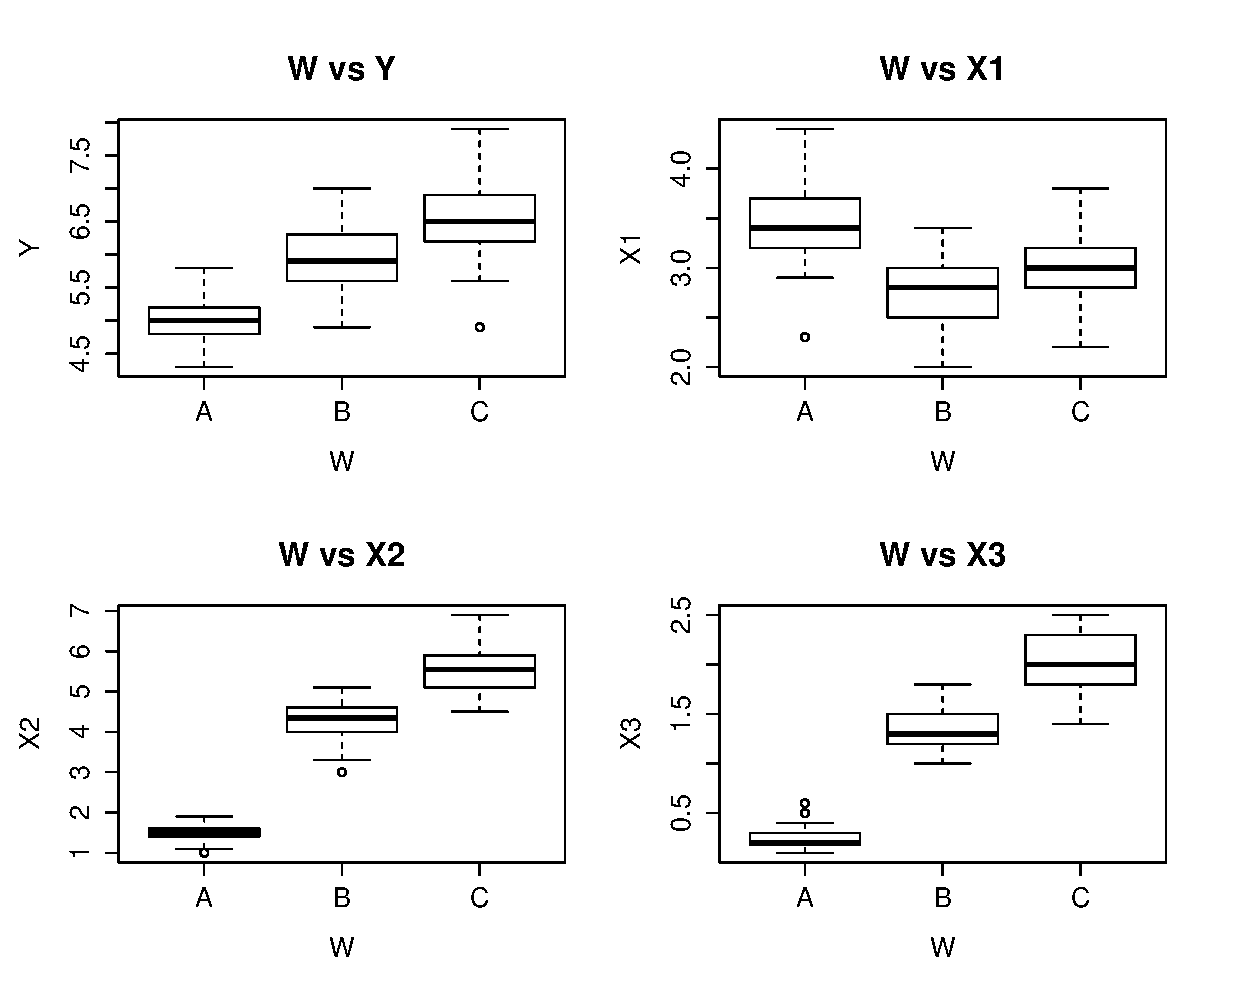
\includegraphics[scale=0.6]{valuesvsW.eps}
\caption{Continuous vs Categorical}
\label{fig:valuesvsW}
\end{figure}

\subsubsection{}
Provide the ANOVA output


\begin{enumerate}
  \item W vs Y
  \begin{lstlisting}
"Fitted model:"
Call:
   aov(formula = data[[col]] ~ factor(W), data = data)

Terms:
                factor(W) Residuals
Sum of Squares   63.21213  38.95620
Deg. of Freedom         2       147

Residual standard error: 0.5147894
Estimated effects may be unbalanced
  \end{lstlisting}
  
  \begin{lstlisting}
"Anova table:"
             Df Sum Sq Mean Sq F value Pr(>F)    
factor(W)     2  63.21  31.606   119.3 <2e-16 ***
Residuals   147  38.96   0.265                   
---
Signif. codes:  0 ‘***’ 0.001 ‘**’ 0.01 ‘*’ 0.05 ‘.’ 0.1 ‘ ’ 1
  \end{lstlisting}
  
  According to the ANOVA table above, the Y variable does not have the same mean
  for all values of W. This is also clear on the plot in figure~\ref{fig:YvsW}
  (p.~\pageref{fig:YvsW}).
  
  \begin{figure}[H]
  \centering
  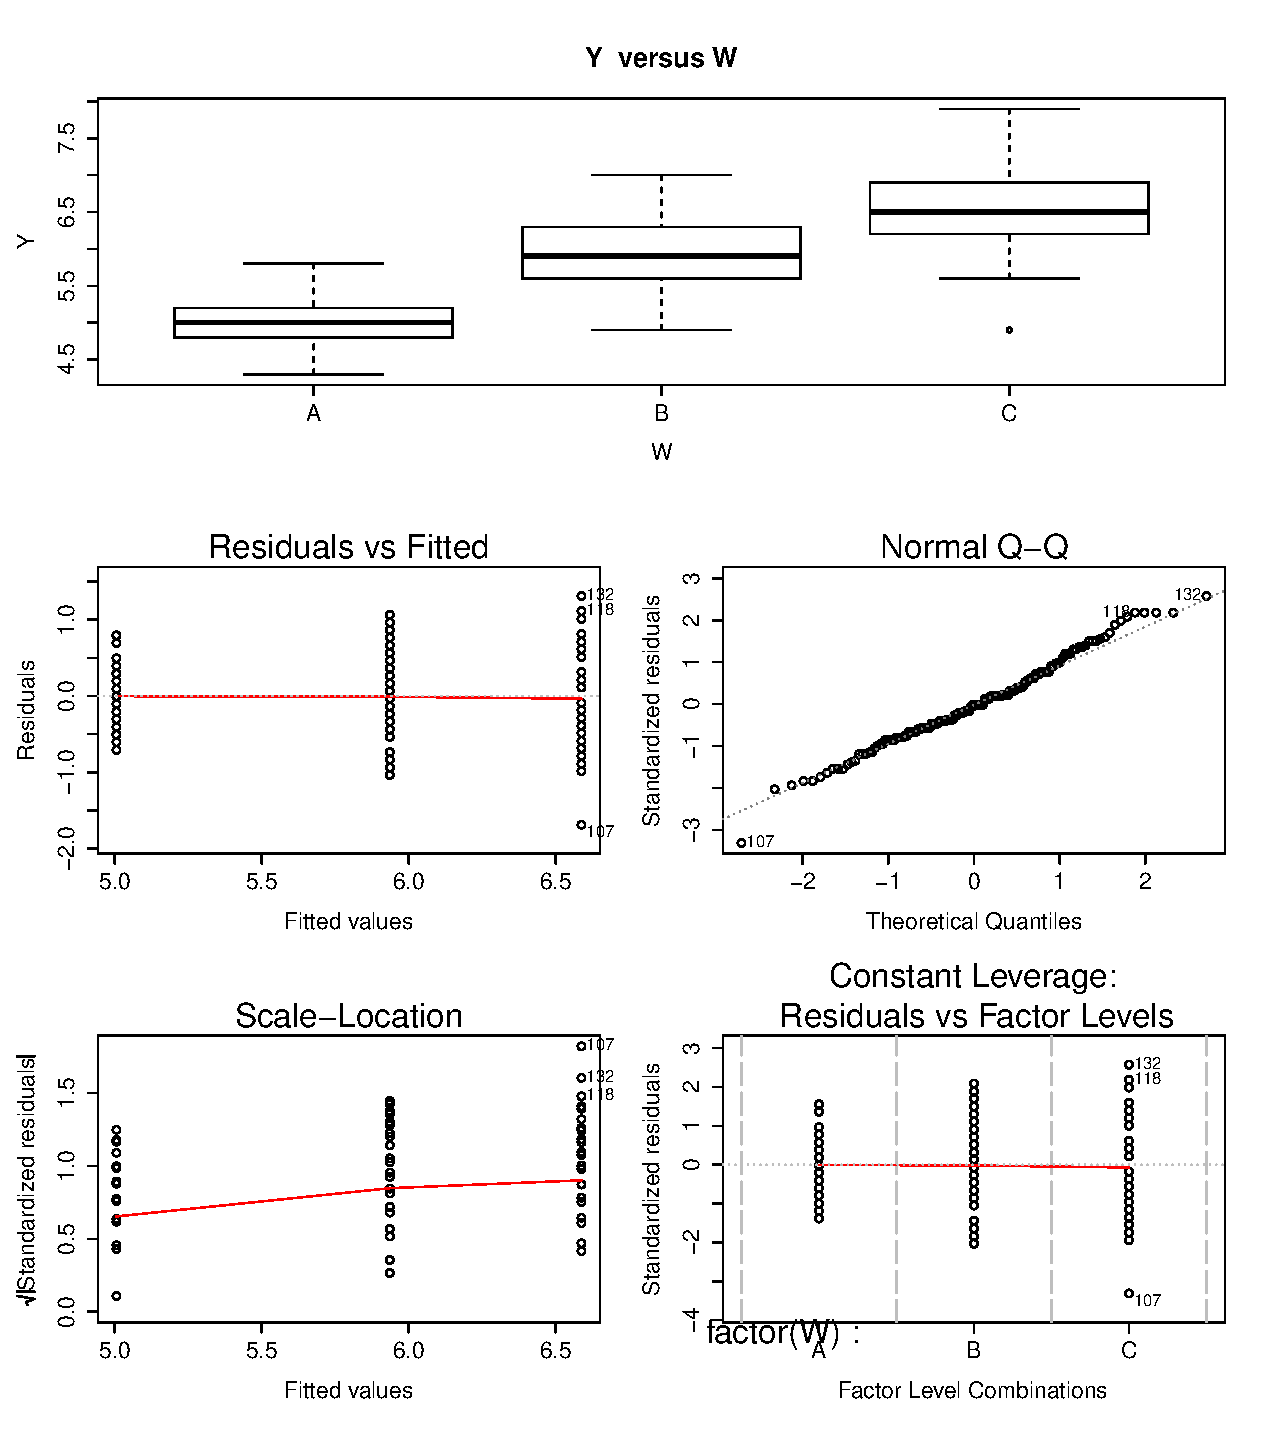
\includegraphics[scale=0.6]{YvsW.eps}
  \caption{W vs Y}
  \label{fig:YvsW}
  \end{figure}

  \item W vs X1
  \begin{lstlisting}
"Fitted model:"
Call:
   aov(formula = data[[col]] ~ factor(W), data = data)

Terms:
                factor(W) Residuals
Sum of Squares   11.34493  16.96200
Deg. of Freedom         2       147

Residual standard error: 0.3396877
Estimated effects may be unbalanced
  \end{lstlisting}
  
  \begin{lstlisting}
"Anova table:"
             Df Sum Sq Mean Sq F value Pr(>F)    
factor(W)     2  11.35   5.672   49.16 <2e-16 ***
Residuals   147  16.96   0.115                   
---
Signif. codes:  0 ‘***’ 0.001 ‘**’ 0.01 ‘*’ 0.05 ‘.’ 0.1 ‘ ’ 1
  \end{lstlisting}
  
  According to the ANOVA table above, the X1 variable does not have the same
  mean for all values of W. This is also clear on the plot in
  figure~\ref{fig:X1vsW} (p.~\pageref{fig:X1vsW}).
  
  \begin{figure}[H]
  \centering
  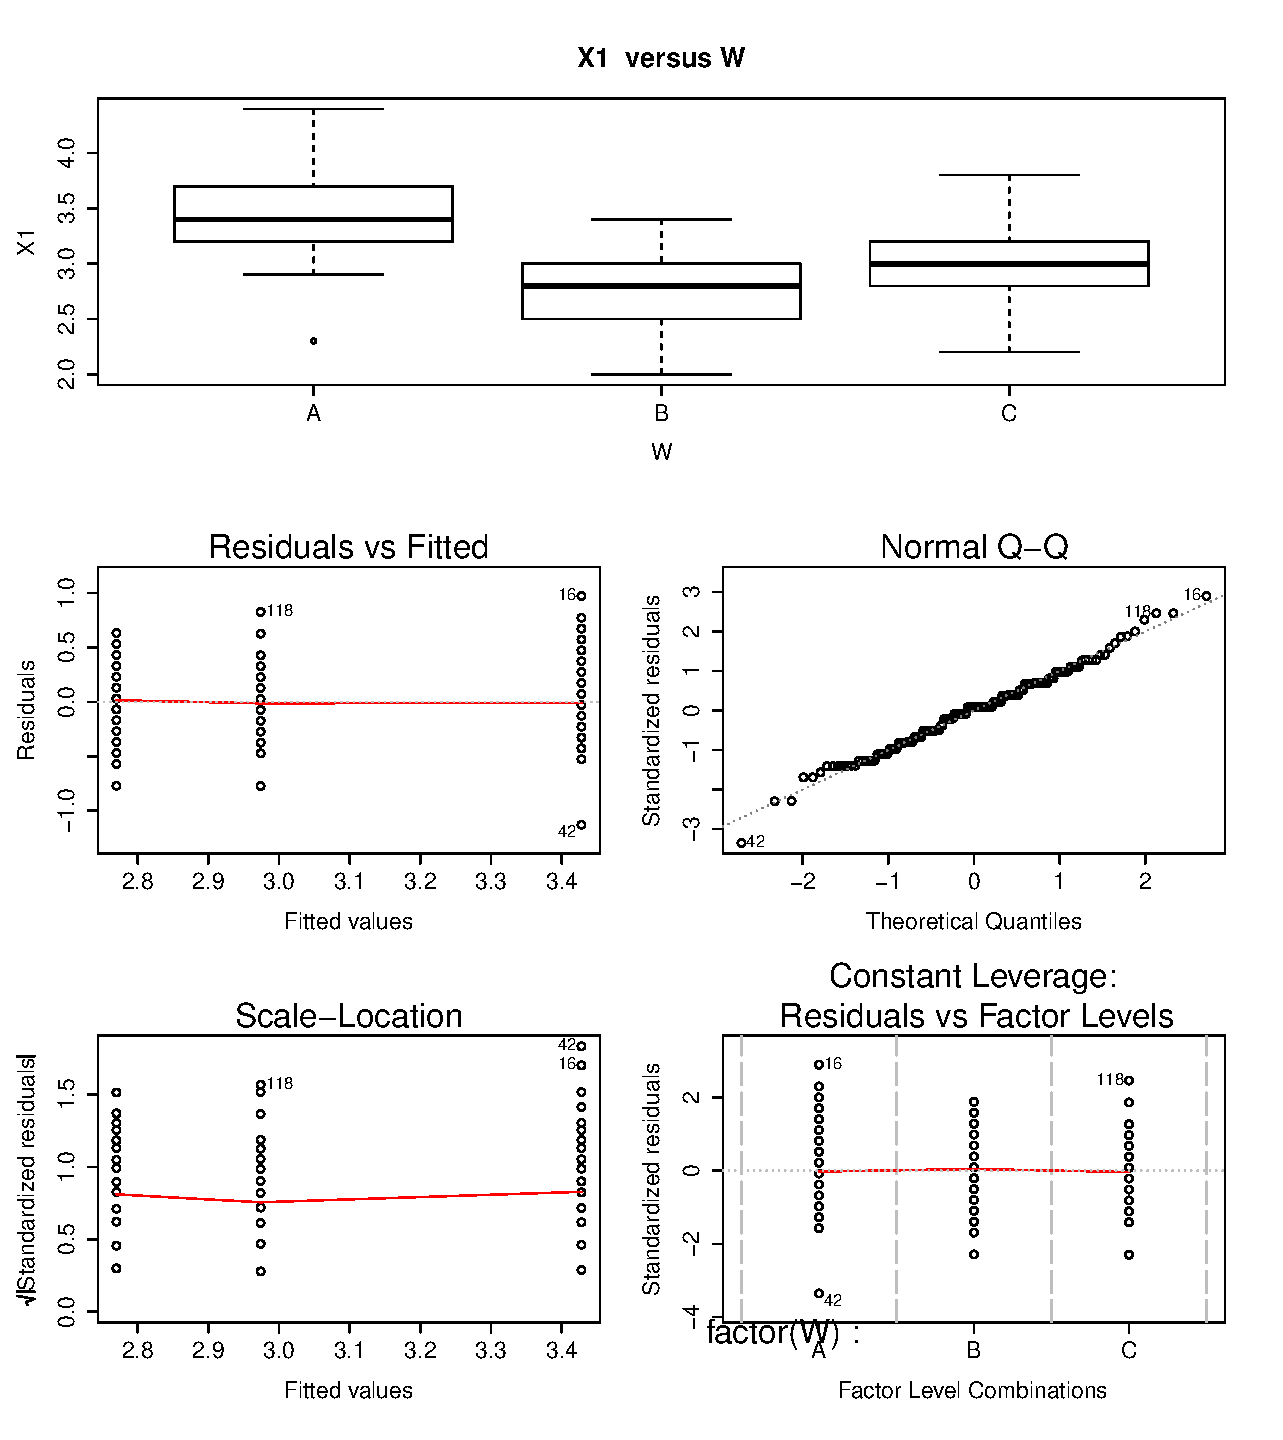
\includegraphics[scale=0.6]{X1vsW.eps}
  \caption{W vs X1}
  \label{fig:X1vsW}
  \end{figure}
  
  \item W vs X2
  \begin{lstlisting}
"Fitted model:"
Call:
   aov(formula = data[[col]] ~ factor(W), data = data)

Terms:
                factor(W) Residuals
Sum of Squares   437.1028   27.2226
Deg. of Freedom         2       147

Residual standard error: 0.4303345
Estimated effects may be unbalanced
  \end{lstlisting}

  \begin{lstlisting}
"Anova table:"
             Df Sum Sq Mean Sq F value Pr(>F)    
factor(W)     2  437.1  218.55    1180 <2e-16 ***
Residuals   147   27.2    0.19                   
---
Signif. codes:  0 ‘***’ 0.001 ‘**’ 0.01 ‘*’ 0.05 ‘.’ 0.1 ‘ ’ 1
  \end{lstlisting}
  
  According to the ANOVA table above, the X2 variable does not have the same
  mean for all values of W. This is also clear on the plot in
  figure~\ref{fig:X2vsW} (p.~\pageref{fig:X2vsW}).
  
  \begin{figure}[H]
  \centering
  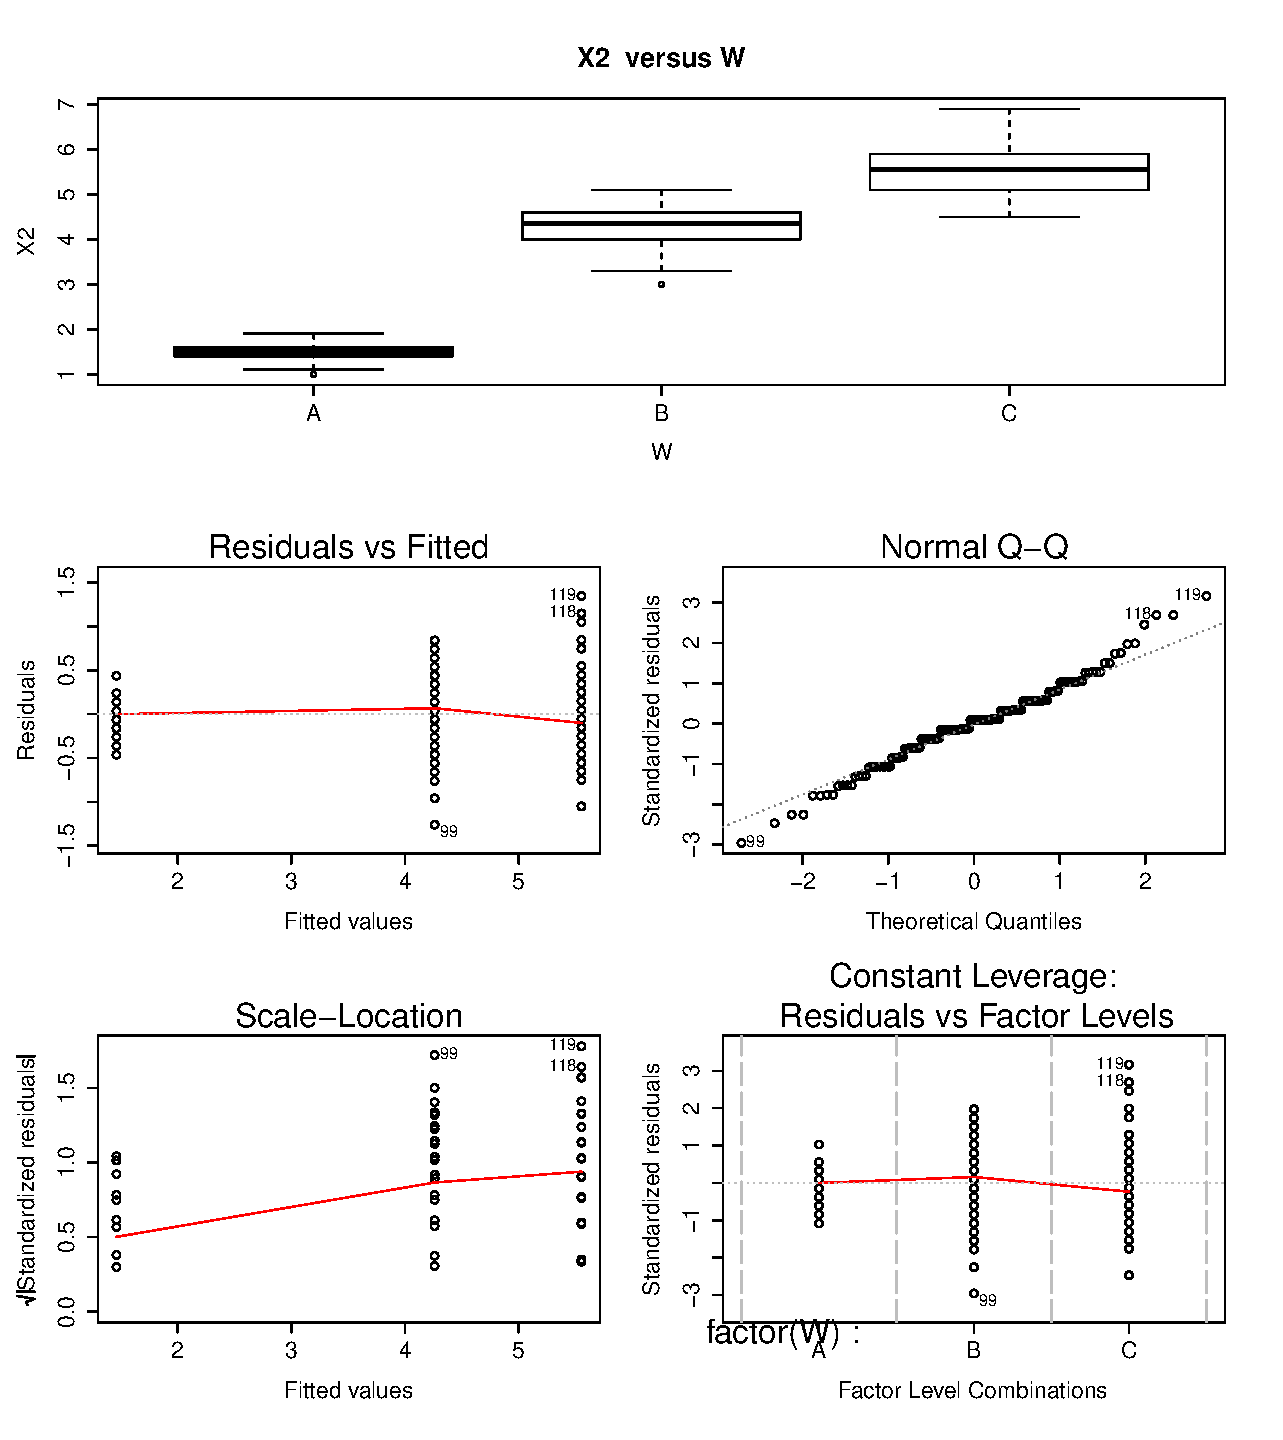
\includegraphics[scale=0.6]{X2vsW.eps}
  \caption{W vs X2}
  \label{fig:X2vsW}
  \end{figure}
  
  \item W vs X3
  \begin{lstlisting}
"Fitted model:"
Call:
   aov(formula = data[[col]] ~ factor(W), data = data)

Terms:
                factor(W) Residuals
Sum of Squares   80.41333   6.15660
Deg. of Freedom         2       147

Residual standard error: 0.20465
Estimated effects may be unbalanced
  \end{lstlisting}
  
  \begin{lstlisting}
"Anova table:"
             Df Sum Sq Mean Sq F value Pr(>F)    
factor(W)     2  80.41   40.21     960 <2e-16 ***
Residuals   147   6.16    0.04                   
---
Signif. codes:  0 ‘***’ 0.001 ‘**’ 0.01 ‘*’ 0.05 ‘.’ 0.1 ‘ ’ 1
  \end{lstlisting}
  
  According to the ANOVA table above, the X3 variable does not have the same
  mean for all values of W. This is also clear on the plot in
  figure~\ref{fig:X3vsW} (p.~\pageref{fig:X3vsW}).
  
  \begin{figure}[H]
  \centering
  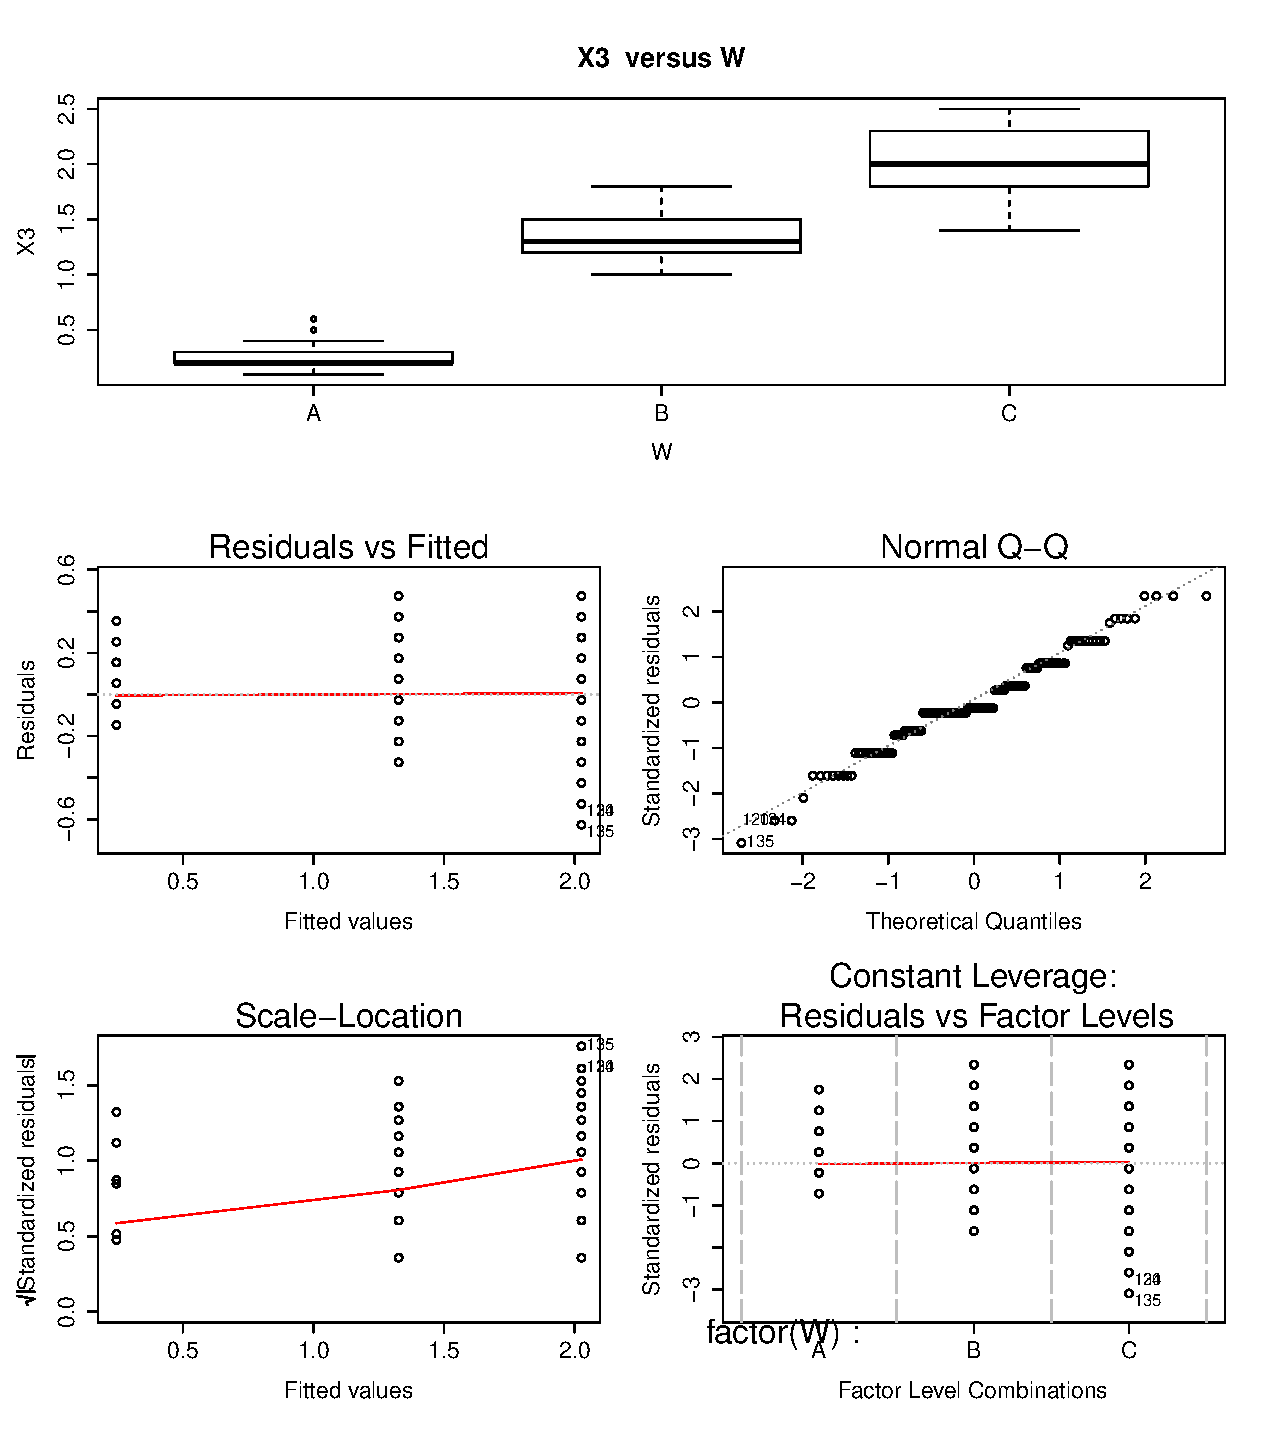
\includegraphics[scale=0.6]{X3vsW.eps}
  \caption{W vs X3}
  \label{fig:X3vsW}
  \end{figure}
\end{enumerate}

\subsubsection{}
Check the assumptions and provide alternatives when the assumptions are violated

\begin{enumerate}
  \item W vs Y
  We will use the Shapiro-Wilk test to check the normality of the residuals:
  \begin{lstlisting}
"Shapiro-Wilk test for normality of residuals:"

	Shapiro-Wilk normality test

data:  fit$residuals
W = 0.9879, p-value = 0.2189
  \end{lstlisting}
  
  The test confirms what we see on the NPP plot in figure~\ref{fig:YvsW}; the
  residuals are from a normal distribution.
  
  Next we will check the homogenity of the variance among the diffrerent values
  of W with the Bartlett test:
  \begin{lstlisting}
"Homogenity of variances:"

	Bartlett test of homogeneity of variances

data:  data[[col]] by factor(W)
Bartlett's K-squared = 16.006, df = 2, p-value = 0.0003345
  \end{lstlisting}
  
  The test reports that the variance is not the same and we can also observe
  that on the box and leverage plot in figure~\ref{fig:YvsW}.
  
  \item W vs X1
  We will use the Shapiro-Wilk test to check the normality of the residuals:
  \begin{lstlisting}
"Shapiro-Wilk test for normality of residuals:"

	Shapiro-Wilk normality test

data:  fit$residuals
W = 0.98948, p-value = 0.323
  \end{lstlisting}
  The test confirms what we see on the NPP plot in figure~\ref{fig:X1vsW}; the
  residuals are from a normal distribution.
  
  Next we will check the homogenity of the variance among the diffrerent values
  of W with the Bartlett test:
  \begin{lstlisting}
"Homogenity of variances:"

	Bartlett test of homogeneity of variances

data:  data[[col]] by factor(W)
Bartlett's K-squared = 2.0911, df = 2, p-value = 0.3515
  \end{lstlisting}
  The test reports that the variance is the same thus the assumptions for the
  analysis of variance are correct.
  
  \item W vs X2
  We will use the Shapiro-Wilk test to check the normality of the residuals:
  \begin{lstlisting}
"Shapiro-Wilk test for normality of residuals:"

	Shapiro-Wilk normality test

data:  fit$residuals
W = 0.98108, p-value = 0.03676
  \end{lstlisting}
  The test indicates that the residuals are not normally distributed.
  
  Next we will check the homogenity of the variance among the diffrerent values
  of W with the Bartlett test:
  \begin{lstlisting}
"Homogenity of variances:"

	Bartlett test of homogeneity of variances

data:  data[[col]] by factor(W)
Bartlett's K-squared = 5
  \end{lstlisting}
  The test reports that the variance is not the same and we can also observe
  that on the box and leverage plot in figure~\ref{fig:X2vsW}.
  
  \item W vs X3
  We will use the Shapiro-Wilk test to check the normality of the residuals:
  \begin{lstlisting}
"Shapiro-Wilk test for normality of residuals:"

	Shapiro-Wilk normality test

data:  fit$residuals
W = 0.97217, p-value = 0.003866
  \end{lstlisting}
  The test indicates that the residuals are not normally distributed.
  
  Next we will check the homogenity of the variance among the diffrerent values
  of W with the Bartlett test:  
  \begin{lstlisting}
"Homogenity of variances:"

	Bartlett test of homogeneity of variances

data:  data[[col]] by factor(W)
Bartlett's K-squared = 39.213, df = 2, p-value = 3.055e-09
  \end{lstlisting}
  The test reports that the variance is not the same and we can also observe
  that on the box and leverage plot in figure~\ref{fig:X3vsW}.
\end{enumerate}

\subsubsection{}
If significant mean diferences exist, then use two different ad-hoc methods to
identify the mean grouping versus the levels of the categorical variable

\begin{enumerate}
  \item W vs Y
  The mean differences are significant in this case. We will use the Tukey
  honestly significant differences method and the pairwiase t-test to identify
  the difference in means:
  \begin{lstlisting}
Tukey multiple comparisons of means
    95% family-wise confidence level

Fit: aov(formula = data[[col]] ~ factor(W), data = data)

$`factor(W)`
     diff       lwr       upr p adj
B-A 0.930 0.6862273 1.1737727     0
C-A 1.582 1.3382273 1.8257727     0
C-B 0.652 0.4082273 0.8957727     0
  \end{lstlisting}
  
  \begin{lstlisting}
	Pairwise comparisons using t tests with pooled SD 

data:  data[["Y"]] and data[["W"]] 

  A       B      
B 1.8e-15 -      
C < 2e-16 2.8e-09

P value adjustment method: holm 
  \end{lstlisting}
  
  \item W vs X1
  The mean differences are significant in this case. We will use the Tukey
  honestly significant differences method and the pairwiase t-test to identify
  the difference in means:
  \begin{lstlisting}
  Tukey multiple comparisons of means
    95% family-wise confidence level

Fit: aov(formula = data[[col]] ~ factor(W), data = data)

$`factor(W)`
      diff         lwr        upr     p adj
B-A -0.658 -0.81885528 -0.4971447 0.0000000
C-A -0.454 -0.61485528 -0.2931447 0.0000000
C-B  0.204  0.04314472  0.3648553 0.0087802
  \end{lstlisting}
  
  \begin{lstlisting}
	Pairwise comparisons using t tests with pooled SD 

data:  data[["X1"]] and data[["W"]] 

  A       B     
B < 2e-16 -     
C 9.1e-10 0.0031

P value adjustment method: holm
  \end{lstlisting}
  
  \item W vs X2
  The mean differences are significant in this case. We will use the Tukey
  honestly significant differences method and the pairwiase t-test to identify
  the difference in means:
  \begin{lstlisting}
  Tukey multiple comparisons of means
    95% family-wise confidence level

Fit: aov(formula = data[[col]] ~ factor(W), data = data)

$`factor(W)`
     diff     lwr     upr p adj
B-A 2.798 2.59422 3.00178     0
C-A 4.090 3.88622 4.29378     0
C-B 1.292 1.08822 1.49578     0
  \end{lstlisting}
  
  \begin{lstlisting}
	Pairwise comparisons using t tests with pooled SD 

data:  data[["X2"]] and data[["W"]] 

  A      B     
B <2e-16 -     
C <2e-16 <2e-16

P value adjustment method: holm 
  \end{lstlisting}
  
  \item W vs X3
  The mean differences are significant in this case. We will use the Tukey
  honestly significant differences method and the pairwiase t-test to identify
  the difference in means:
  \begin{lstlisting}
  Tukey multiple comparisons of means
    95% family-wise confidence level

Fit: aov(formula = data[[col]] ~ factor(W), data = data)

$`factor(W)`
    diff       lwr       upr p adj
B-A 1.08 0.9830903 1.1769097     0
C-A 1.78 1.6830903 1.8769097     0
C-B 0.70 0.6030903 0.7969097     0
  \end{lstlisting}
  
  \begin{lstlisting}
	Pairwise comparisons using t tests with pooled SD 

data:  data[["X3"]] and data[["W"]] 

  A      B     
B <2e-16 -     
C <2e-16 <2e-16

P value adjustment method: holm
  \end{lstlisting}
\end{enumerate}

\subsection{}
Run the non-parametric one-way ANOVA of each of the continuous variables ($Y,
X_1, X_2, X_3$) on the categorical variable ($W$)

The Kruskal-Wallis is the non-parametric one-way ANOVA test.
\begin{enumerate}
  \item W vs Y
  \begin{lstlisting}
  	Kruskal-Wallis rank sum test

data:  data[["Y"]] by data[["W"]]
Kruskal-Wallis chi-squared = 96.937, df = 2, p-value < 2.2e-16
  \end{lstlisting}
  \item W vs X1
  \begin{lstlisting}
	Kruskal-Wallis rank sum test

data:  data[["X1"]] by data[["W"]]
Kruskal-Wallis chi-squared = 63.571, df = 2, p-value = 1.569e-14
  \end{lstlisting}
  \item W vs X2
  \begin{lstlisting}
	Kruskal-Wallis rank sum test

data:  data[["X2"]] by data[["W"]]
Kruskal-Wallis chi-squared = 130.41, df = 2, p-value < 2.2e-16
  \end{lstlisting}
  \item W vs X3
  \begin{lstlisting}
	Kruskal-Wallis rank sum test

data:  data[["X3"]] by data[["W"]]
Kruskal-Wallis chi-squared = 131.19, df = 2, p-value < 2.2e-16
  \end{lstlisting}
\end{enumerate}

\subsection{}
Provide a scatter-plot matrix of $Y, X_1, X_2, X_3$
  \begin{figure}[H]
  \centering
  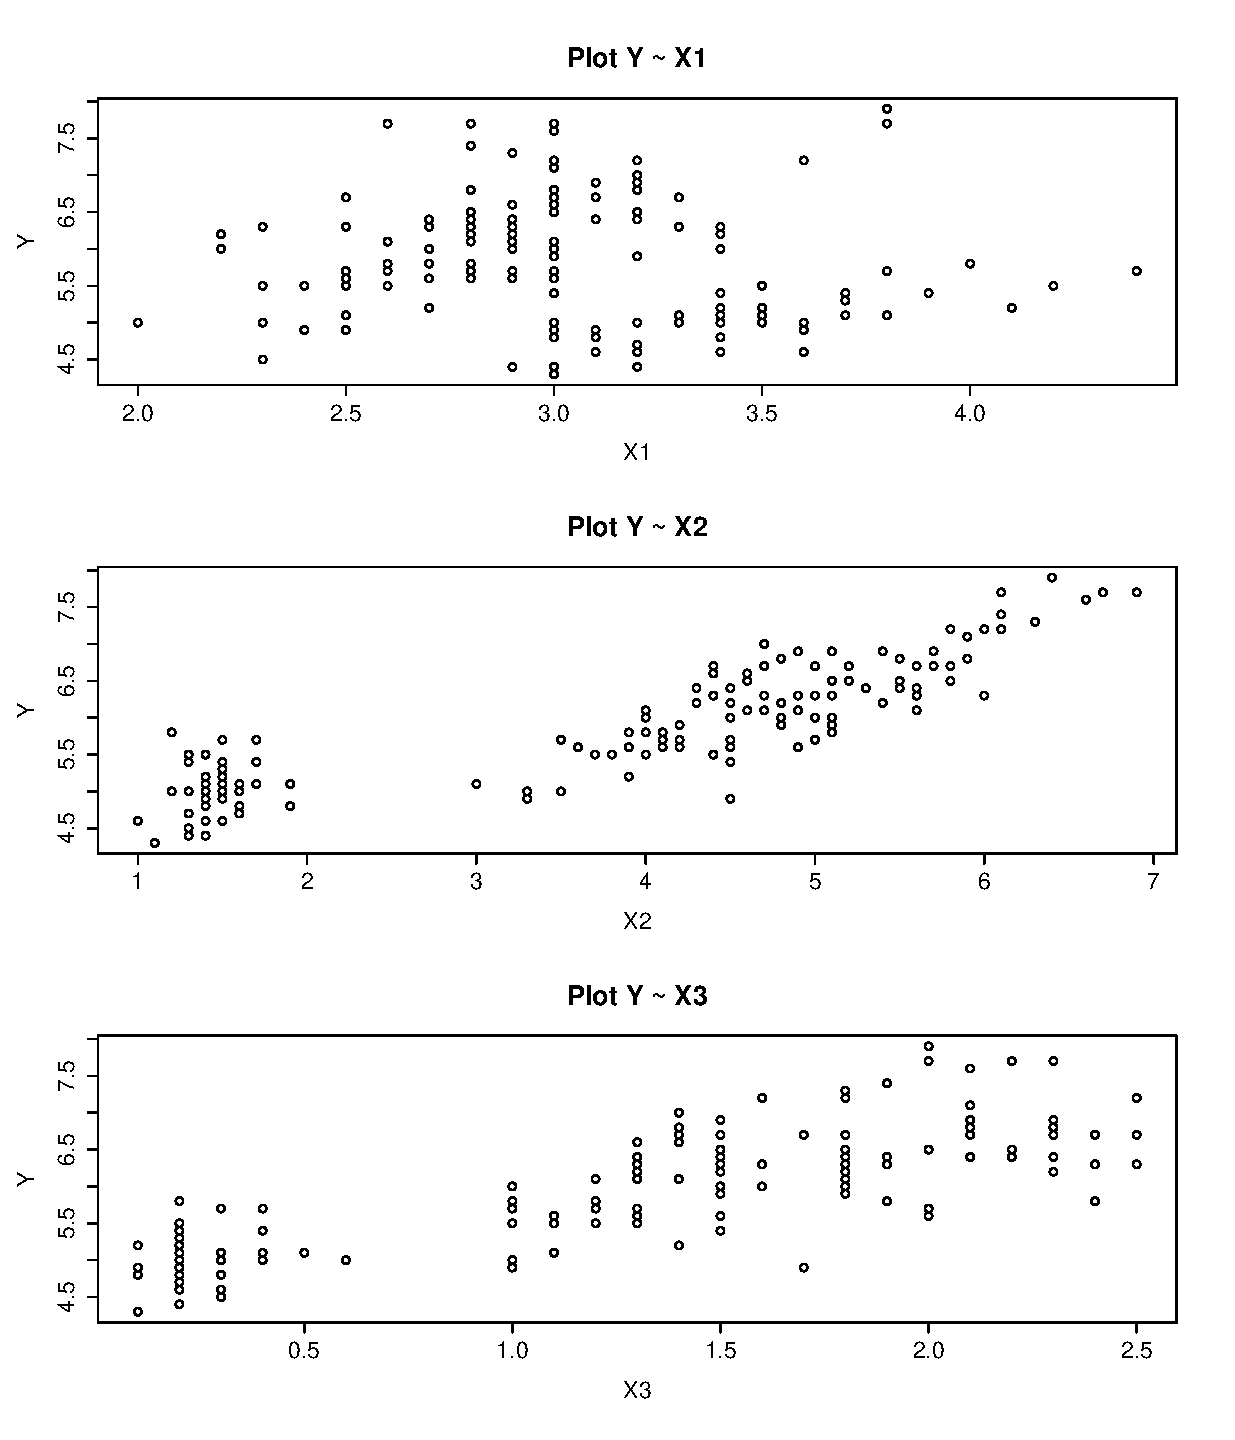
\includegraphics[scale=0.6]{scatter.eps}
  \caption{Scatter plot of continuous variables}
  \label{fig:scatter}
  \end{figure}

\subsection{}
Provide a scatter-plot matrix of $Y, X_1, X_2, X_3$, annotating the different
levels of W in each plot using a different color.

  \begin{figure}[H]
  \centering
  \includegraphics[scale=0.6]{scattercolors.eps}
  \caption{Scatter plot of continuous variables with coloured levels of W}
  \label{fig:scattercolors}
  \end{figure}

\end{document}
